\documentclass[twocolumn]{article}
\usepackage{amsmath}
\usepackage{amsfonts}
\usepackage{amssymb}
\usepackage{amsbsy}
\usepackage{graphicx}
\usepackage[a4paper,margin=1in]{geometry}

\begin{document}
\section{Case2}
We will study two types of simple model error with Lorenz 96 model. We will introduce constant deterministic error to the standard Lorenz 96 model and try to use ensemble Kalman filter on an augmented system to improve the performance of data assimilation.
\subsection{Notation}
\begin{tabular}{rl}
True model:& $m$\\
Forecast model:& $\hat{m}$\\
True state:& $\pmb{x}_n$\\
Model state:& $\hat{\pmb{x}}_n$\\
Observation Operator:& $H:\pmb{x}_n\mapsto\pmb{y}_n$
\end{tabular}\\
The Lorenz96 equation is:
\begin{equation}
\dot{x_i}=(x_{i+1}-x_{i+2})x_{i-1}-x_{i}+F,\quad i=1,2,...,N
\end{equation}
We will use the common choice of $N=40$ and $F=8$ with periodic boundary conditions. For readability, we write the whole system as:
\begin{equation} \label{lorenz}
\pmb{\dot{x}}=\pmb{L}(\pmb{x})
\end{equation}
\subsection{Types of error}
We consider three types of model error, where the true systems are as follows:
\begin{align} 
\dot{\pmb{x}}=&\pmb{L}(\pmb{x})+\pmb{\zeta} 
&&\mathrm{(Type\quad I)}& \label{error1} \\
\dot{\pmb{x}}=&\pmb{L}(\pmb{x}+\pmb{\xi}) 
&&\mathrm{(Type\quad II)}&\label{error2} \\
\dot{\pmb{x}}=&\pmb{L}(\pmb{x}+\pmb{\xi})+\pmb{\zeta} 
&&\mathrm{(Type\quad III)}& \label{error3}
\end{align}
The first type error is a constant bias. The second type of error models the situation where the true dynamics and the dynamics used for forecasting are associated with a coordinate transformation. For simplicity, we assume the transformation is just a shift of the forecast state to the true state. We combine the two types of error to get the third type of truth bias.\\
For simplicity, we assume that $\pmb{\zeta}$ and $\pmb{\xi}$ in the equations above are both constant in time. Some have suggested that when the error is arguably small, they exhibit behaviors similar to those of the system. Accordingly, we set
\begin{align}
\zeta_i=&A\sin(2\pi\dfrac{i-1}{N}) \label{Adef} \\
\xi_i=&B\sin(2\pi\dfrac{i-1}{N}),\quad i=1,...,N \label{Bdef}
\end{align}
where $A$ and $B$ are constants.\\
\subsection{Model} \label{models}
The true model $m$ used for generating the truth is integrating eq.(\ref{error1},\ref{error2},\ref{error3}), respectively in each setting, from time $t_{n-1}$ to time $t_{n}$. The forecast model $\hat{m}$ used for evolving the model state is integrating eq.(\ref{lorenz}) from time $t_{n-1}$ to time $t_{n}$.\\
In the numerical experiments below, to avoid the potential influence of error introduced by numerical integration, we do not use a fixed step method for integration. Instead, we use an error correction method with a specified error tolerance of $10^{-7}$. One common method of such type is fourth order Runge-Kutta method, with a fifth order Runge-Kutta method used for error estimation. In Matlab, it's ode45.
\subsubsection{Model 1} \label{model1}
To address the Type I model error, we first define the model bias:
\begin{equation}
\pmb{b}_{n}=m(\pmb{x}_{n-1})-\hat{m}(\pmb{x}_{n-1})
\end{equation}
We therefore incorporate $\pmb{b}_n$ to the augmented system:
\begin{align}
\pmb{x}_{n}^{f}=&\hat{m}(\pmb{x}_{n-1}^{a})+\pmb{b}_{n}^{f}\\
\pmb{b}_{n}^{f}=&f_{b}(\pmb{x}_{n-1}^{a},\pmb{b}_{n}^{a})
\end{align}
In the case where $\pmb{\zeta}$ is constant, we assume $\pmb{b}_n$ is constant too, and then
\begin{equation}
\pmb{b}_{n}^{f}=f_{b}(\pmb{x}_{n-1}^{a},\pmb{b}_{n-1}^{a})=\pmb{b}_{n-1}^{a}
\end{equation}
To see how this model associates with the Type I error, we suppose the model state and true state are close, i.e. the bias is small, and then take the difference between the true equation (\ref{error1}) and the model equation (\ref{lorenz}),
\begin{equation} \label{M1Diff}
\dfrac{d}{dt}(\pmb{x}-\hat{\pmb{x}})=\pmb{L}(\pmb{x})+\pmb{\zeta}-\pmb{L}(\hat{\pmb{x}})\approx\pmb{\zeta}
\end{equation}
then, integrating eq.(\ref{M1Diff}) for the time interval $t_{n-1}\leq t\leq t_n$ with the initial condition $\pmb{x}(t_{n-1})=\hat{\pmb{x}}(t_{n-1})=\pmb{x}_{n-1}$, to obtain the following
\begin{equation} \label{b&zeta}
\pmb{b}_n=\pmb{x}(t_{n})-\hat{\pmb{x}}(t_{n})\approx\int_{t_{n-1}}^{t_n}\pmb{\zeta}dt=\pmb{\zeta}\Delta t
\end{equation}
Since $\pmb{\zeta}$ is constant in time, if the data assimilation scheme works, then the augmented state $pmb{b}_n$ should converge to a value that is very close to $\pmb{\zeta}\Delta t$. In the numerical experiments below, we will therefore compare time averaged $pmb{b}_n$ and $\pmb{\zeta}\Delta t$ to see if the bias estimation is successful.
\subsubsection{Model 2} \label{model2}
For the second type of error, we use the analysis to model $\hat{\pmb{x}}_n$ instead of the true state $\pmb{x}_n$. We define the bias as
\begin{equation}
\pmb{c}_{n}=m(\pmb{x}_{n-1}^{t})-\hat{m}(\pmb{x}_{n-1}^{m})=m(\pmb{x}_{n-1}^{t})-\hat{m}(\pmb{x}_{n-1}^{t}-\pmb{c}_{n-1})
\end{equation}
The augmented system then becomes
\begin{align}
\pmb{x}_{n}^{f}=&\hat{m}(\pmb{x}_{n-1}^{a})\\
\pmb{c}_{n}^{f}=&f_{c}(\pmb{x}_{n-1}^{a},\pmb{c}_{n}^{a})
\end{align}
For simplicity, we assume we know $\pmb{\xi}$ is constant, which means $\pmb{c}_n$ should be constant, and then
\begin{equation}
\pmb{c}_{n}^{f}=f_{c}(\pmb{x}_{n-1}^{a},\pmb{c}_{n-1}^{a})=\pmb{c}_{n-1}^{a}
\end{equation} 
Note that in such setting, the analysis will model the model trajectory $\hat{\pmb{x}}_{n}$ instead of the true trajectory $\pmb{x}_n$, and therefore the observation should be:
\begin{equation}
\pmb{y}_n=H(\hat{\pmb{x}}_n+\pmb{c}_n)
\end{equation}
To see how the augmented state $\pmb{c}$ relates to the model error $\pmb{\xi}$, we differentiate $\pmb{c}$ to get
\begin{equation} \label{c&xi}
\begin{split}
\dfrac{d\pmb{c}}{dt}&=\dfrac{d\pmb{x}}{dt}-\dfrac{d\hat{\pmb{x}}}{dt}\\
&=\pmb{L}(\pmb{x}+\pmb{\xi})-\pmb{L}(\hat{\pmb{x}})\\
&=\pmb{L}(\pmb{x}+\pmb{\xi})-\pmb{L}(\pmb{x}-\pmb{c})
\end{split}
\end{equation}
Apparently, $\pmb{c}=-\pmb{\xi}$ solves the equation, and therefore it's reasonable to believe if our data assimilation works, $\pmb{c}$ will converge to $-\pmb{\xi}$. In the numerical experiments below, we will thus compare a time averaged $\pmb{c}$ and $-\pmb{\xi}$ to see if the bias estimation is successful.
\subsubsection{Model 3} \label{model3}
When we combine the two types of the model errors and try to address them together, we have the following scheme:
\begin{align}
\pmb{x}_{n}^{f}=&\hat{m}(\pmb{x}_{n-1}^{a})+\pmb{b}_{n}^{f}\\
\pmb{b}_{n}^{f}=&f_{b}(\pmb{x}_{n-1}^{a},\pmb{b}_{n-1}^{a},\pmb{c}_{n-1}^{a})\\
\pmb{c}_{n}^{f}=&f_{c}(\pmb{x}_{n-1}^{a},\pmb{b}_{n-1}^{a},\pmb{c}_{n-1}^{a})
\end{align}
Again, for simplicity, we assume $c_n$ and $b_n$ are constant, i.e.,
\begin{align}
\pmb{b}_{n}^{f}=&f_{b}(\pmb{x}_{n-1}^{a},\pmb{b}_{n-1}^{a})=\pmb{b}_{n-1}^{a}\\
\pmb{c}_{n}^{f}=&f_{c}(\pmb{x}_{n-1}^{a},\pmb{c}_{n-1}^{a})=\pmb{c}_{n-1}^{a}
\end{align}
Same as in Model 2, the observation operator becomes
\begin{equation}
\pmb{y}_n=H(\hat{\pmb{x}}_n+\pmb{c}_n)
\end{equation}
Since model 3 is simply a combination of model 1 and 2, it's natural to reason that $\pmb{b}\approx\pmb{\zeta}\Delta t$ and $\pmb{c}=-\pmb{\xi}$ still hold. Indeed, if we differentiate $\pmb{b}$, we have
\begin{equation}
\dfrac{d\pmb{b}}{dt}=\pmb{L}(\pmb{x}+\pmb{\xi})+\pmb{\zeta}-\pmb{L}(\pmb{x}-\pmb{c})
\end{equation}
which gives us solution
\begin{align}
\dfrac{d\pmb{b}}{dt}=\pmb{\zeta}\Rightarrow\pmb{b}&=\pmb{\zeta}\Delta t\\
\pmb{c}&=-\pmb{\xi}
\end{align}
which is consistent with our reasoning for model 1 and 2.
\subsection{Numerical Experiments}
\subsubsection{Experiment Setup}
In each setting of error, we will use ensemble Kalman Filter with perfect model assumption, i.e. without an augmented system, and with Model 1, 2, and 3, to estimate the solution. We will compare the performance of these different methods.\\
In order for ensemble Kalman filter to work, we will introduce uncorrelated Gaussian noise with zero mean and $\sigma_{obs}=0.09$ at each step to the observation operator.\\
We will use time-averaged root-mean-square of the analysis error to measure the performance of the different methods, where the analysis error of Model 1 is defined as
\begin{equation}
\bar{\pmb{e}}^{(n)}_a=\bar{\pmb{x}}_n^a-\pmb{x}_n,
\end{equation}
and the analysis error of Model 2 and 3 is
\begin{equation}
\bar{\pmb{e}}^{(n)}_a=\bar{\pmb{x}}_n^a+\bar{\pmb{c}}_n-\pmb{x}_n,
\end{equation}
where $\bar{\pmb{x}}_n^a$ is the ensemble mean of the analysis at each step and $\bar{\pmb{c}}_n$ the ensemble mean of the bias $\pmb{c}_n$. And root-mean-square of the analysis error is denoted as $\langle\bar{\pmb{e}}_a^{(n)}\rangle$, the time-average $\langle\langle\bar{\pmb{e}}_a^{(n)}\rangle\rangle$.\\
To improve the analyses in our experiments, we employ variance inflation
\begin{equation} \label{inflation}
\pmb{P}_n^a\rightarrow \pmb{P}_n^a+\dfrac{\mu\Lambda}{K}\pmb{I}_K
\end{equation}
where $\pmb{P}_n^a$ is the analysis error covariance matrix, $\mu$ is an inflation coefficient, whose value is critical to the performance of data assimilation, which we will discuss below, $\Lambda =\mathrm{Trace}(\pmb{P}_n^a)$, $K$ is the dimension of the augmented space for each model, and $\pmb{I}_k$ is the $K$ dimensional identity matrix. 
\subsubsection{Effect of Randomness}
The experiments are in some sense not deterministic, since, first, the observations are generated with white noise, second, we introduce randomness in the initial state of the ensemble and we randomly perturb the observations at each step. Some have suggested using averaged results over trials with various random seeds instead of results of an individual trial to avoid the possibility that, in some extreme cases, the randomness might lead to abnormal behavior of the results. Nevertheless, after many experiments with different random seeds and everything else fixed, we found no significant differences worth mentioning in the results. Therefore we will simply use the results of a single trial, in each of the settings below.
\subsubsection{Effect of Ensemble Size}
Considering the dimension of the problem $N=40$, to also use $M=40$ as ensemble size seems a rational choice. On the one hand, it's natural to assume the reasonable choice of ensemble size is proportional to the dimension of the problem. On the other hand, to make the ensemble size larger than or equal to the dimension of the system largely avoids the rank deficiency of the covariance matrix.\\
After some experiments, we found that, in each setting of model error, for the model that best captures the model error, the ensemble size does not significantly affect the performance of data assimilation. Meanwhile, for the models that do not capture the model error well and the model without bias estimation, increased ensemble size might improve the performance of data assimilation. Fig.(\ref{AErrVsEns}) demonstrates the relation between the performance of data assimilation and the choice of ensemble size.
\begin{figure} 
\centering
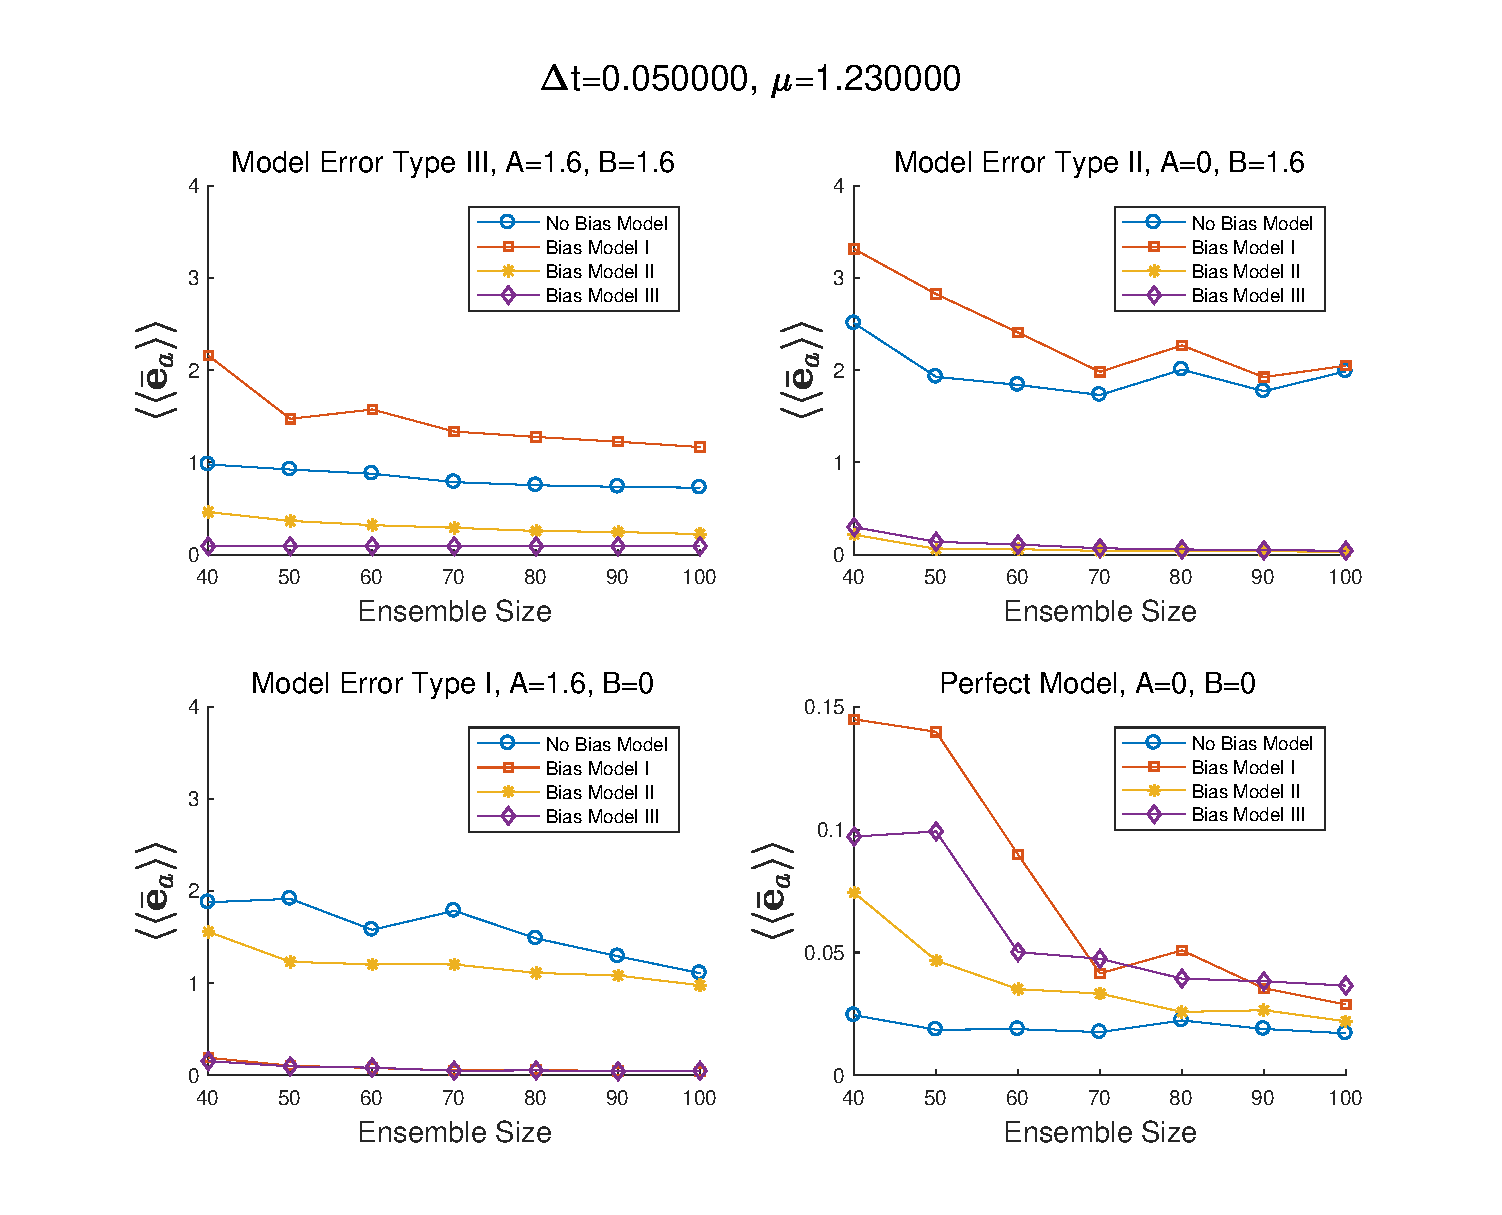
\includegraphics[scale=0.3]{Figures/AErrVsEns1}
\caption{Time-averaged rms analysis error, $\langle\langle\bar{\pmb{e}}_a\rangle\rangle$, versus ensemble size $M$, for the different cases of model error, each with all 4 models.}
\label{AErrVsEns}
\end{figure}\\
Some research has suggested choosing different ensemble sizes for each of the models. For example, choose ensemble size proportional to the dimension of the augmented space, i.e. $M$ for perfect model, $2M$ for model 1 and 2, and $3M$ for model 3.\\
However, such approach would potentially mix the effects of successful bias estimation with increased ensemble size. Also, since ensemble size is not a significant factor in increasing performance, we will choose an ensemble size of $M=40$ for all the models in the experiments below.
\subsubsection{Effect of Step Size}
Many sources have suggested using $\Delta t=0.05$ as the step size between two observations. Nevertheless, it's interesting to inspect how the step size $\Delta t$ influence the performance of data assimilation. Intuitively speaking, the more frequent we make the observations, the better the performance should be.\\
As shown in Fig.(\ref{AErrVsDeltaT1}), the performance is not significantly affected by step size, similar to the case of ensemble size discussed above. We can also see that in some cases, the increase in step size even make the data assimilation worse.
\begin{figure} 
\centering
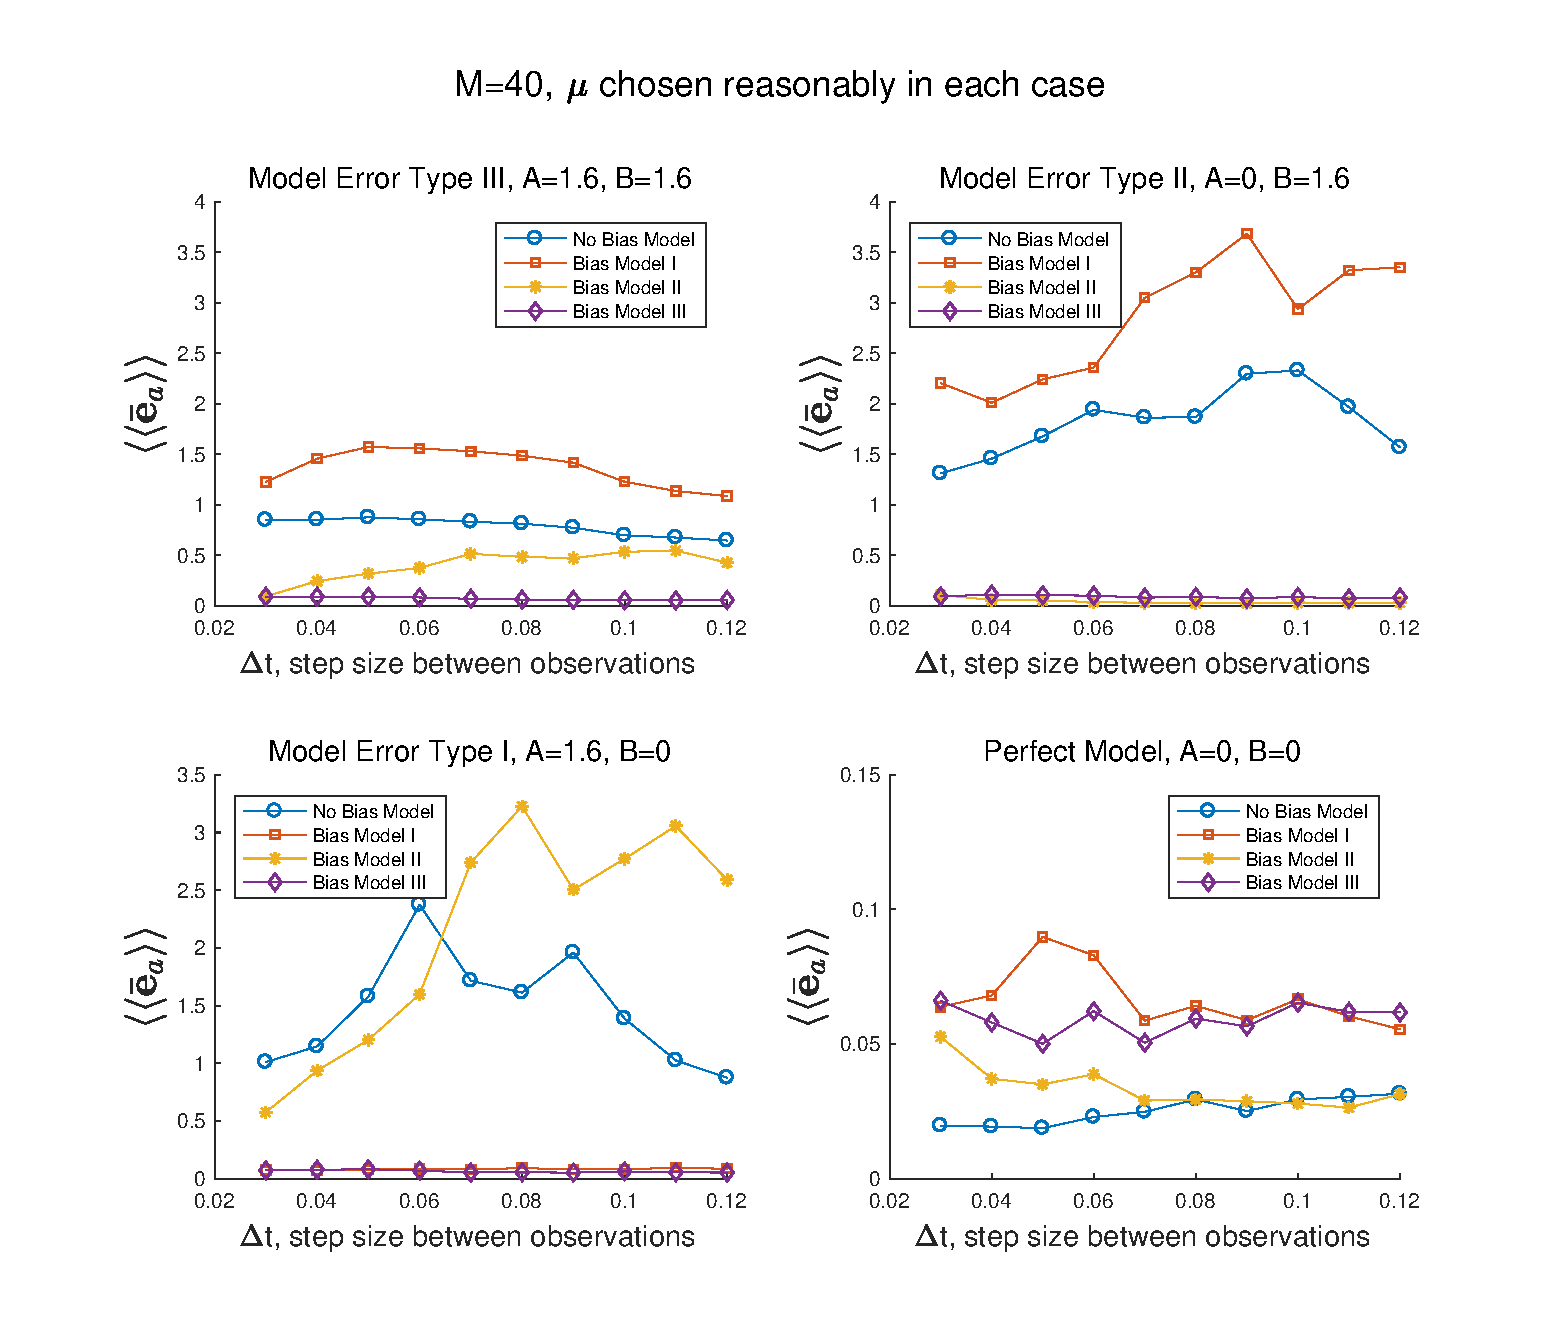
\includegraphics[scale=0.3]{Figures/AErrVsDeltaT1}
\caption{Time-averaged rms analysis error, $\langle\langle\bar{\pmb{e}}_a\rangle\rangle$, versus step size between observations $\Delta t$, for the different cases of model error, each with all 4 models.}
\label{AErrVsDeltaT1}
\end{figure}\\
Therefore, we will simply use the suggested $\Delta t=0.05$ for the experiments below.
\subsubsection{Effect of Inflation Coefficient} \label{EffMu}
Throughout the experiment, we realize that the most significant factor affecting the performance appears to be the inflation coefficient $\mu$, as defined in eq.(\ref{inflation}). In each of the model error settings, for each of the models, there seems to be an optimal value for $\mu$ to achieve the best performance. Moreover, the relation between performance and the inflation coefficient seems complicated. The optimal values of $\mu$ in each situation for each model are quite different. In some cases, a poorly chosen $\mu$ could make the better model perform worse than other models. Therefore, in the discussion below, we will mainly focus on the relation between the variance inflation parameter $\mu$ and the time averaged rms error $\langle\langle\bar{\pmb{e}}_a\rangle\rangle$, as a measure of the performance of data assimilation.
\subsubsection{Perfect Model}
We first test our bias models for the case of a perfect forecast model, i.e. for the case when $A=0$ in eq.(\ref{Adef}) and $B=0$ in eq.(\ref{Bdef}), and the true model used for evolving the true state is simply eq.(\ref{lorenz}), the same as the model used for forecast.
\paragraph{Settling time of error}
Since the perfect model is, in some sense, the simplest model, it's natural to assume that the rms analysis error will stay around a constant value, after a short period of time. Fig.(\ref{ErrVsTimeP1}) shows that that is indeed the case. The error settles down with roughly 100 time steps for all four models. We then use 200 as number of time steps in the experiment below, and whenever we refer to "time-averaged" we mean time averaged over time step 100 to 200, a rather stable period for the error.
\begin{figure} 
\centering
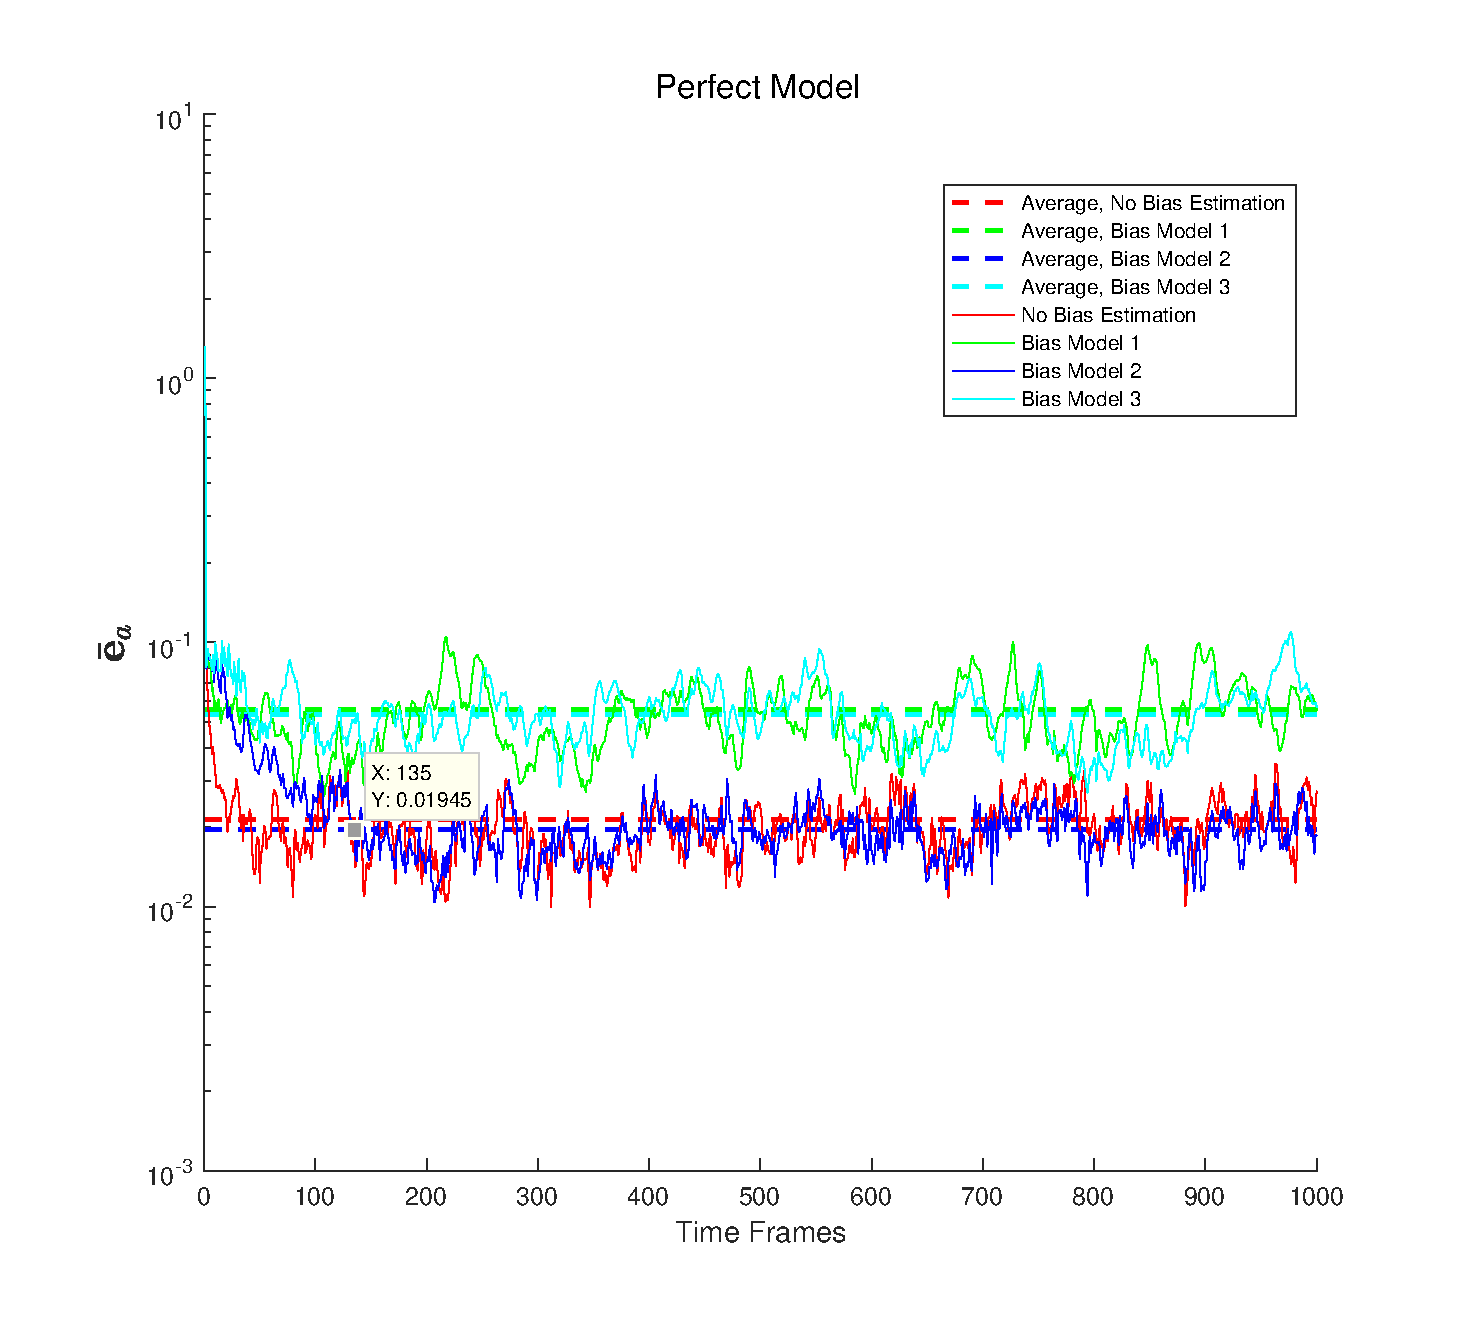
\includegraphics[scale=0.3]{Figures/ErrVsTimeP1}
\caption{Time-averaged rms analysis error, $\langle\langle\bar{\pmb{e}}_a\rangle\rangle$, and rms analysis error at each time step $\bar{\pmb{e}}_a^{(n)}$, for the case without model error, i.e. $A=0,B=0$, with all 4 models.}
\label{ErrVsTimeP1}
\end{figure}
\paragraph{Performance with $\mu$}
As mentioned earlier in section \ref{EffMu}, the most significant factor affecting the performance is the variance inflation coefficient $\mu$. Fig.(\ref{AErrVsMuP1}) shows the relation between error and $\mu$. We can see that, generally speaking, the simple model performs best. This is reasonable, since all other models, in some sense, introduce unnecessary parameters, and the model with the the most unnecessary parameters, i.e. model 3, performs the worst. One interesting phenomena is that for the bias models, the optimal values for $\mu$ are roughly speaking the same, i.e. $\mu=0.378$, and if $\mu$ is larger than this value, the error will increase remarkably.
\begin{figure} 
\centering
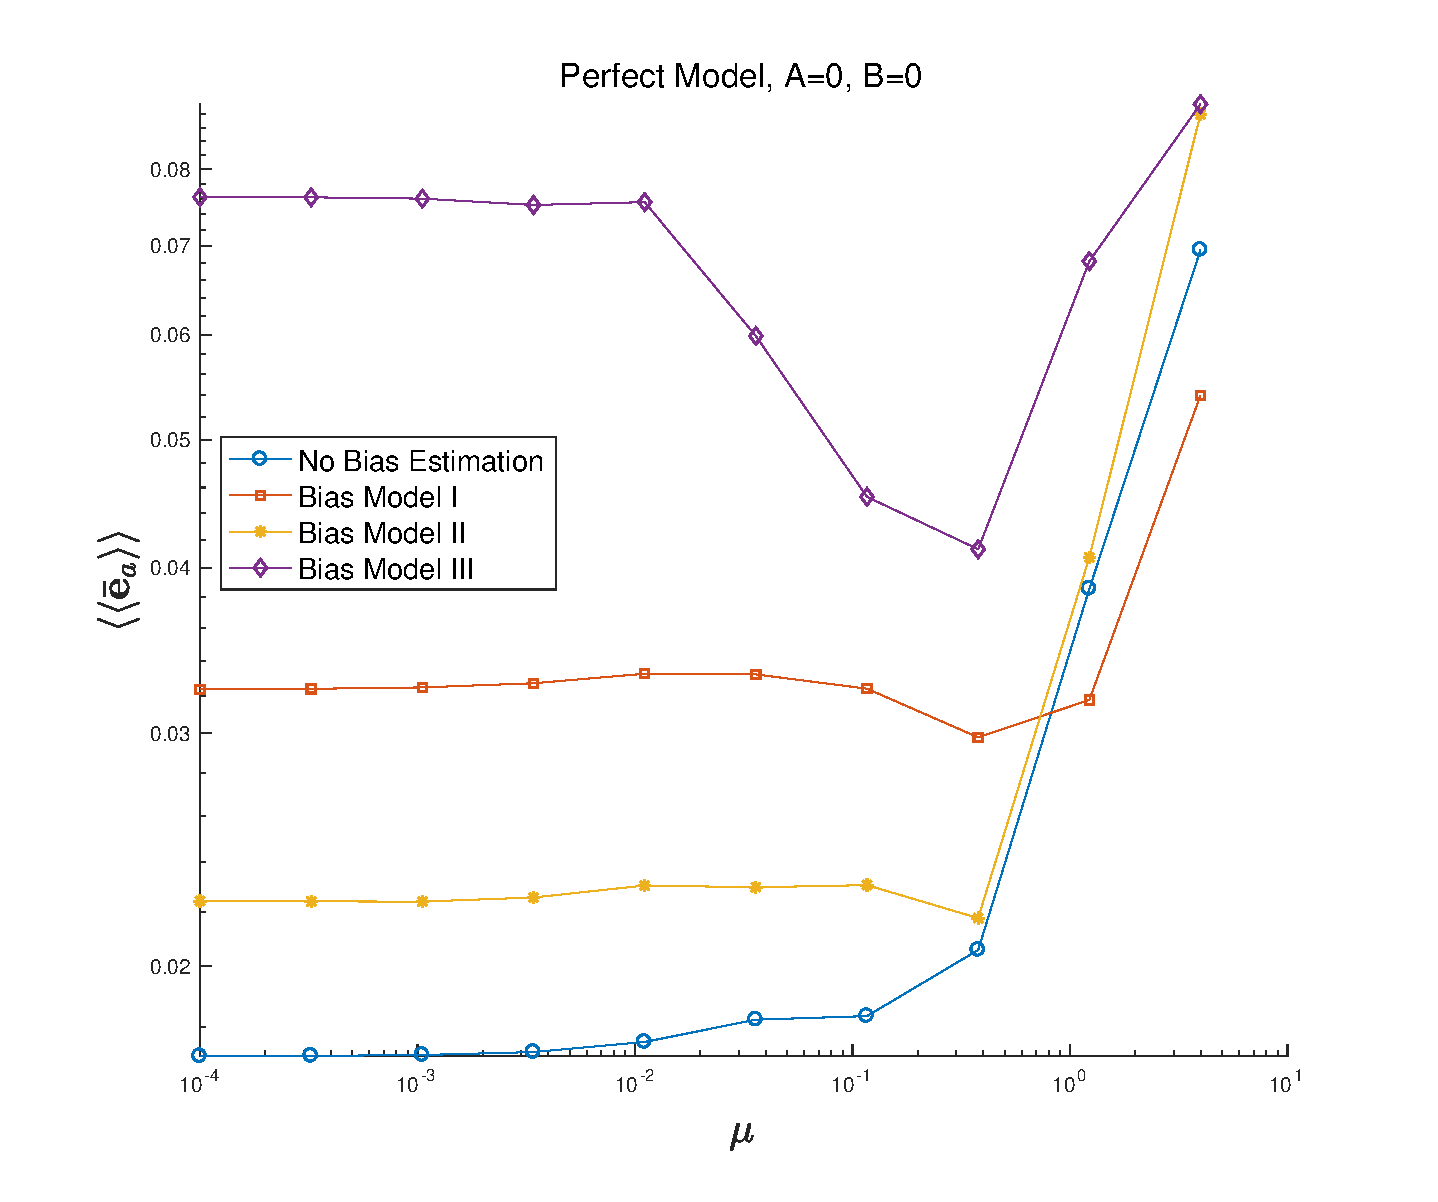
\includegraphics[scale=0.3]{Figures/AErrVsMuP1}
\caption{Time-averaged rms analysis error, $\langle\langle\bar{\pmb{e}}_a\rangle\rangle$, versus the variance inflation parameter $\mu$, for the case without model error, i.e. $A=0,B=0$, with all 4 models.}
\label{AErrVsMuP1}
\end{figure}
\paragraph{Bias estimation}
In this case, the "biases" are simply zero. In Fig.(\ref{BiasEstP1}), we can see that the bias models fail to capture this trivial "bias" very well. Especially for the estimation of $\pmb{c}$, model 2 roughly stays around zero, which is the true value, but model 3 exhibits some unwanted oscillating behavior.
\begin{figure} 
\centering
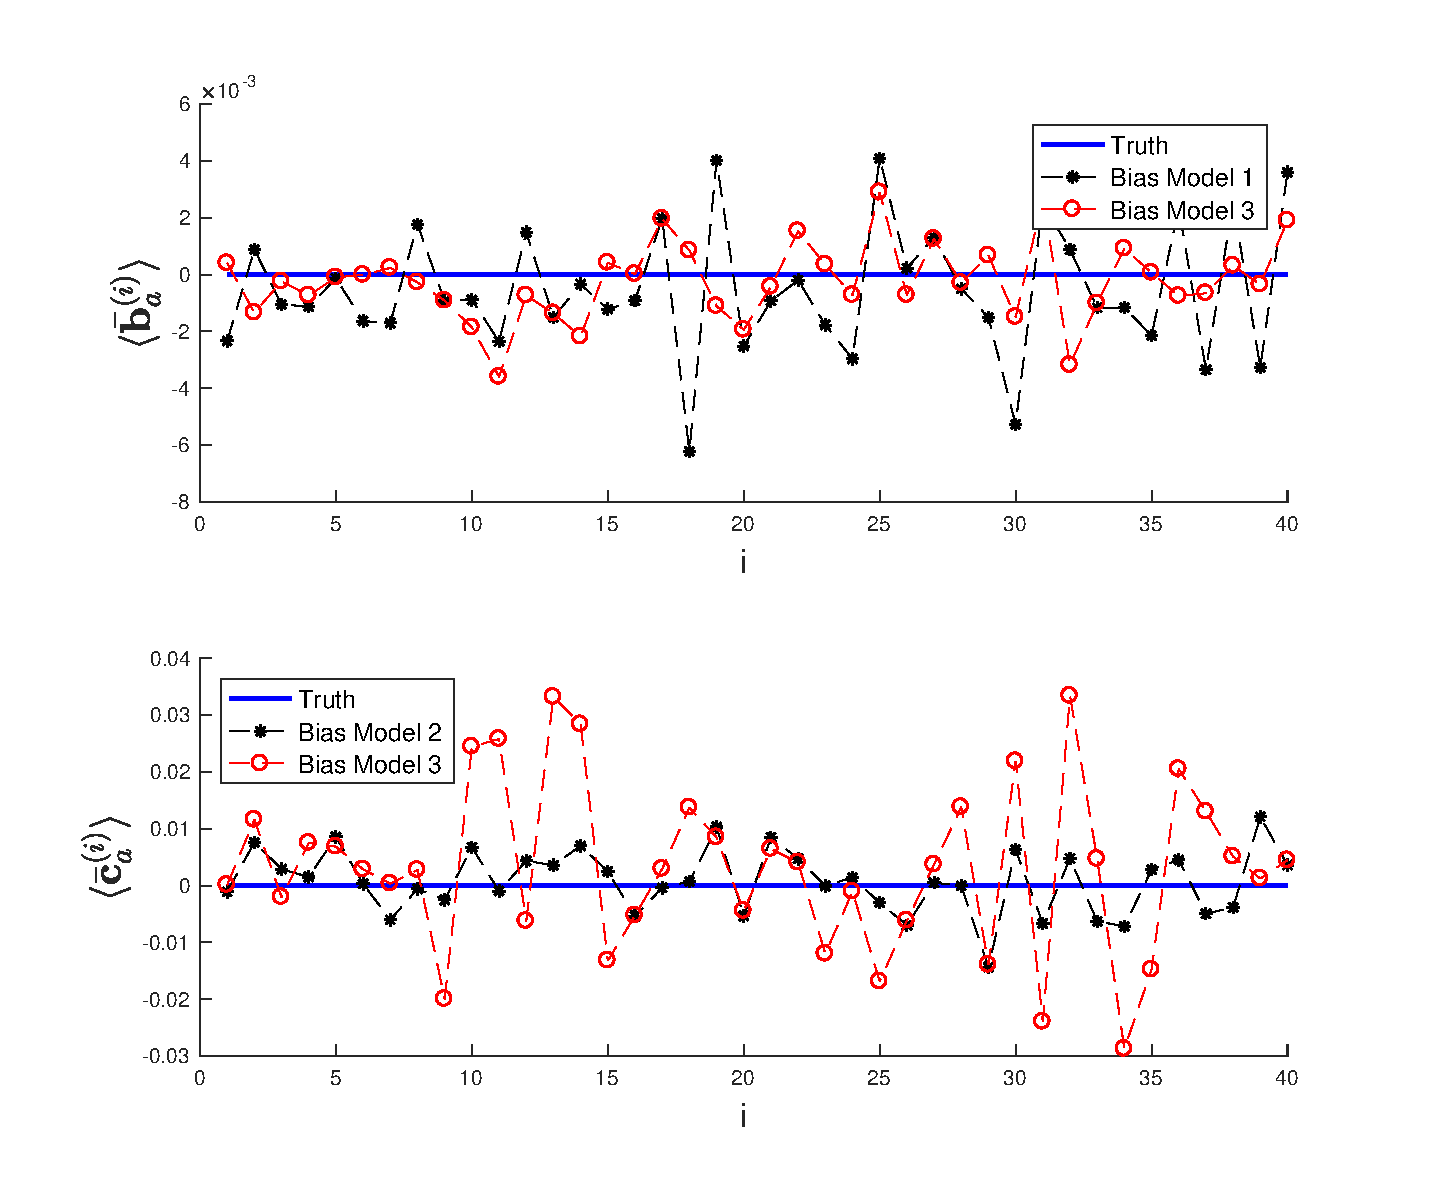
\includegraphics[scale=0.3]{Figures/BiasEstP1}
\caption{Time-averaged bias estimate at each location for the case without model error, i.e. $A=0,B=0$. The truth $\zeta_i\Delta t$ and $-\xi_i$ are shown as the solid curve.}
\label{BiasEstP1}
\end{figure}
\subsubsection{Type I Model Bias}
In this experiment, we perform data assimilation using the model without bias estimation with unaugmented states i.e. eq.(\ref{lorenz}), and the three models with augmented space defined in subsection \ref{models}, when the true state is evolved with Type I model error, defined in eq.(\ref{error1}), with $A=0.2F=1.6$ in eq.(\ref{Adef}).
\paragraph{Settling time of error}
The behavior of error with respect to time in this case is quite different from that of a perfect mode. Fig.(\ref{ErrVsTimeM1.1}) shows that the error for model 1 and 3 converges rather rapidly. However, the errors for the simple model and model 2 are initially small, and then it takes a long time for the errors to stay stable around a value that is considerably large. One way to explain this is that the way model 2 is formulated does not account for this type of model error, and therefore it will not behave very well. We will use 200 as number of time steps in the experiment below, and time step 100 to 200 as the period for time averaging.
\begin{figure} 
\centering
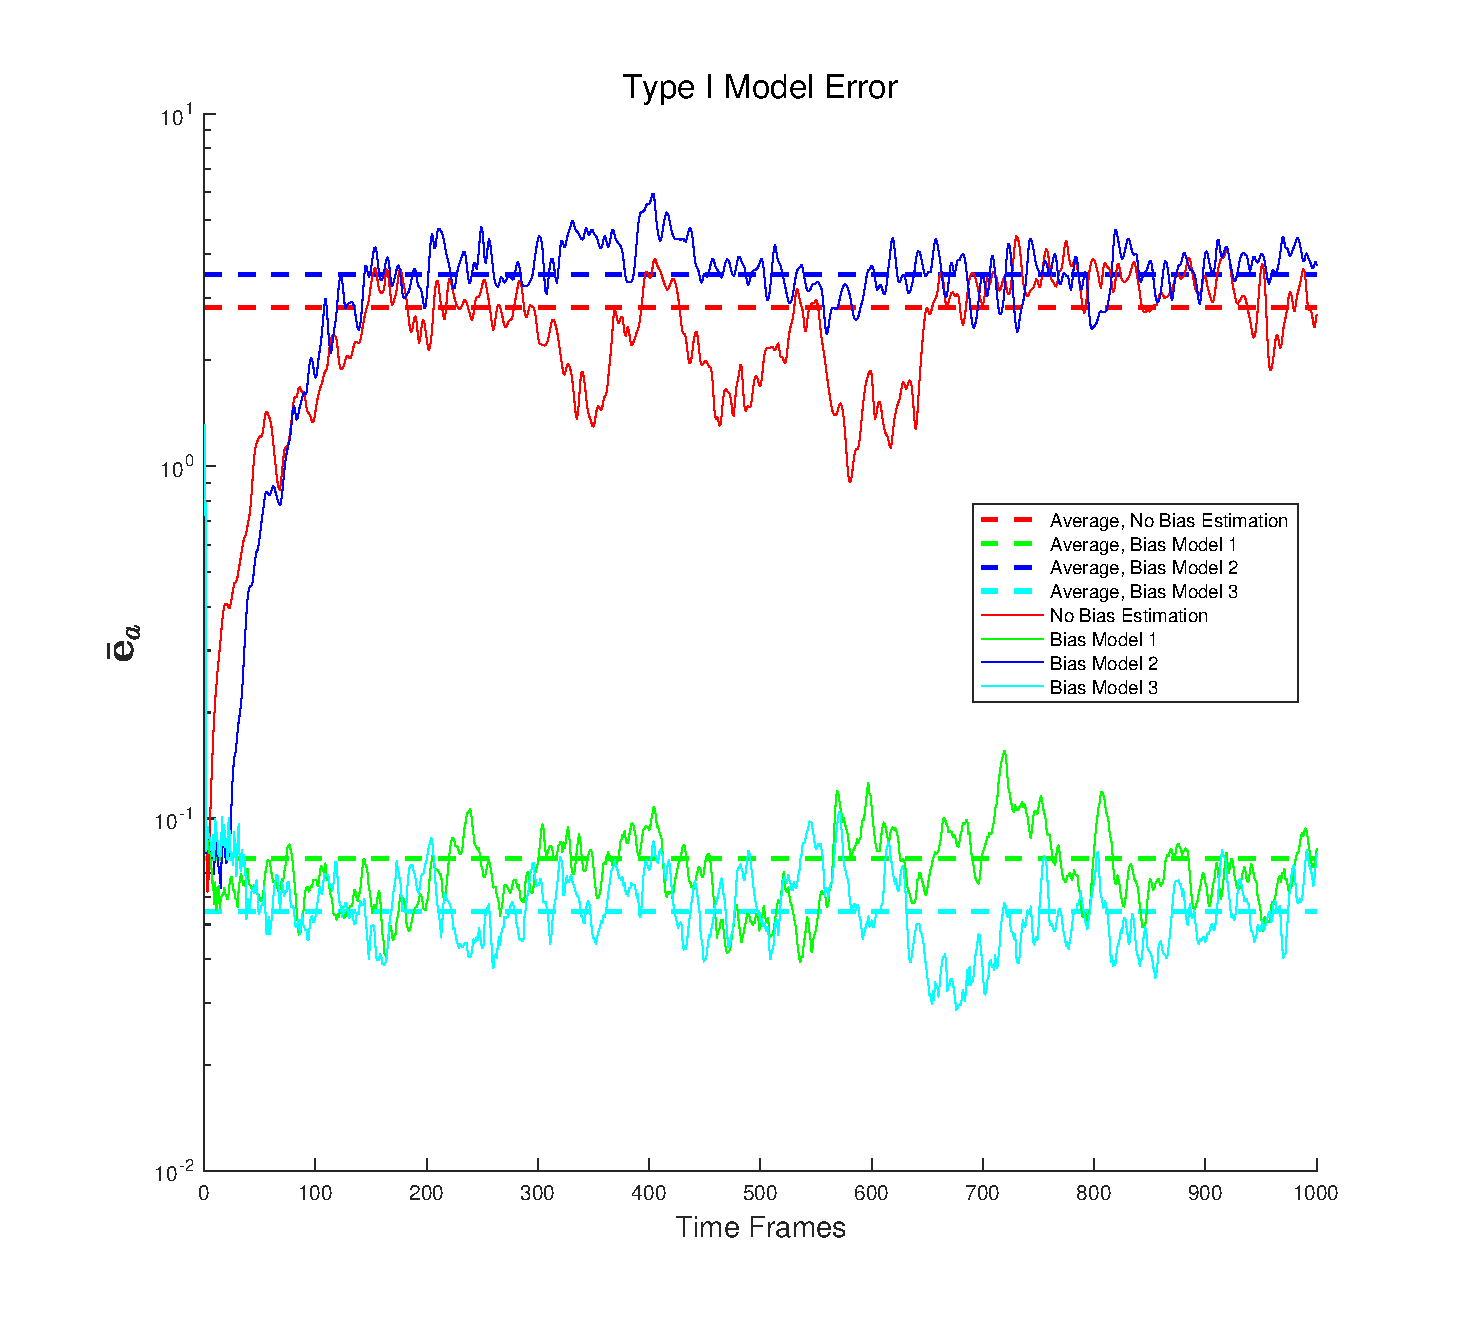
\includegraphics[scale=0.3]{Figures/ErrVsTimeM1_1}
\caption{Time-averaged rms analysis error, $\langle\langle\bar{\pmb{e}}_a\rangle\rangle$, and rms analysis error at each time step $\bar{\pmb{e}}_a^{(n)}$, for the Type I model error, with all 4 models.}
\label{ErrVsTimeM1.1}
\end{figure}
\paragraph{Performance with $\mu$}
Fig.(\ref{AErrVsMuM1.1}) shows the relation between error and $\mu$. Just as we expect, the models that are formulated to account for the Type I model bias perform better than those that do not account for this type of model bias. Model 1 performs the best, and model 3 performs a little bit worse, since model 3 introduces unnecessary parameters $\pmb{b}$ in this case. We can see that for model 1 and 3, the value of $\mu$ does not affect the performance much, especially for model 1. However, for the other two models, larger value of $\mu$ significantly improves the performance, and when $\mu=4$, the model without bias estimation even beats model 3.
\begin{figure} 
\centering
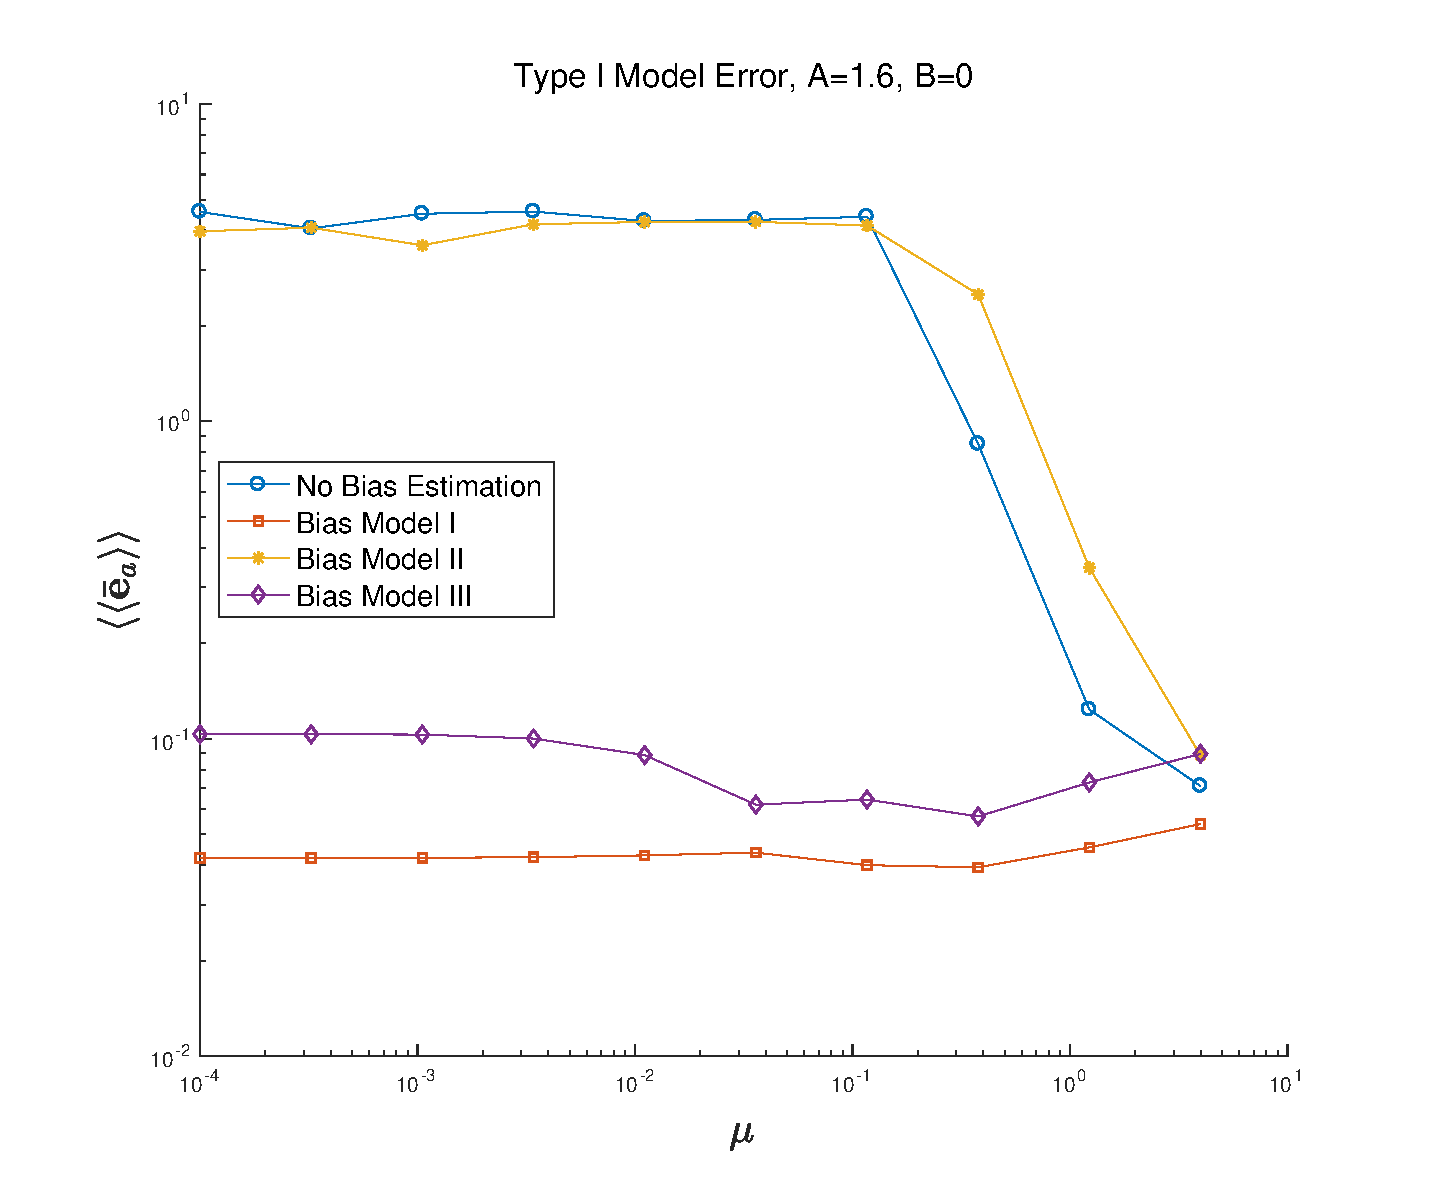
\includegraphics[scale=0.3]{Figures/AErrVsMuM1_1}
\caption{Time-averaged rms analysis error, $\langle\langle\bar{\pmb{e}}_a\rangle\rangle$, versus the variance inflation parameter $\mu$, for the Type I model error, with all 4 models.}
\label{AErrVsMuM1.1}
\end{figure}
\paragraph{Bias estimation}
Fig.(\ref{BiasEstM1}) shows the results for bias estimation. Both model 1 and 3 capture the bias very well, with very few noticeable deviance from the truth. Moreover, unlike the case of perfect model, the estimation for the zero "bias" is successful for model 3, although miserable for model 2. This is very interesting. Heuristically speaking, model 3 is closer to the truth than model 2, and therefore estimates the zero bias better.
\begin{figure} 
\centering
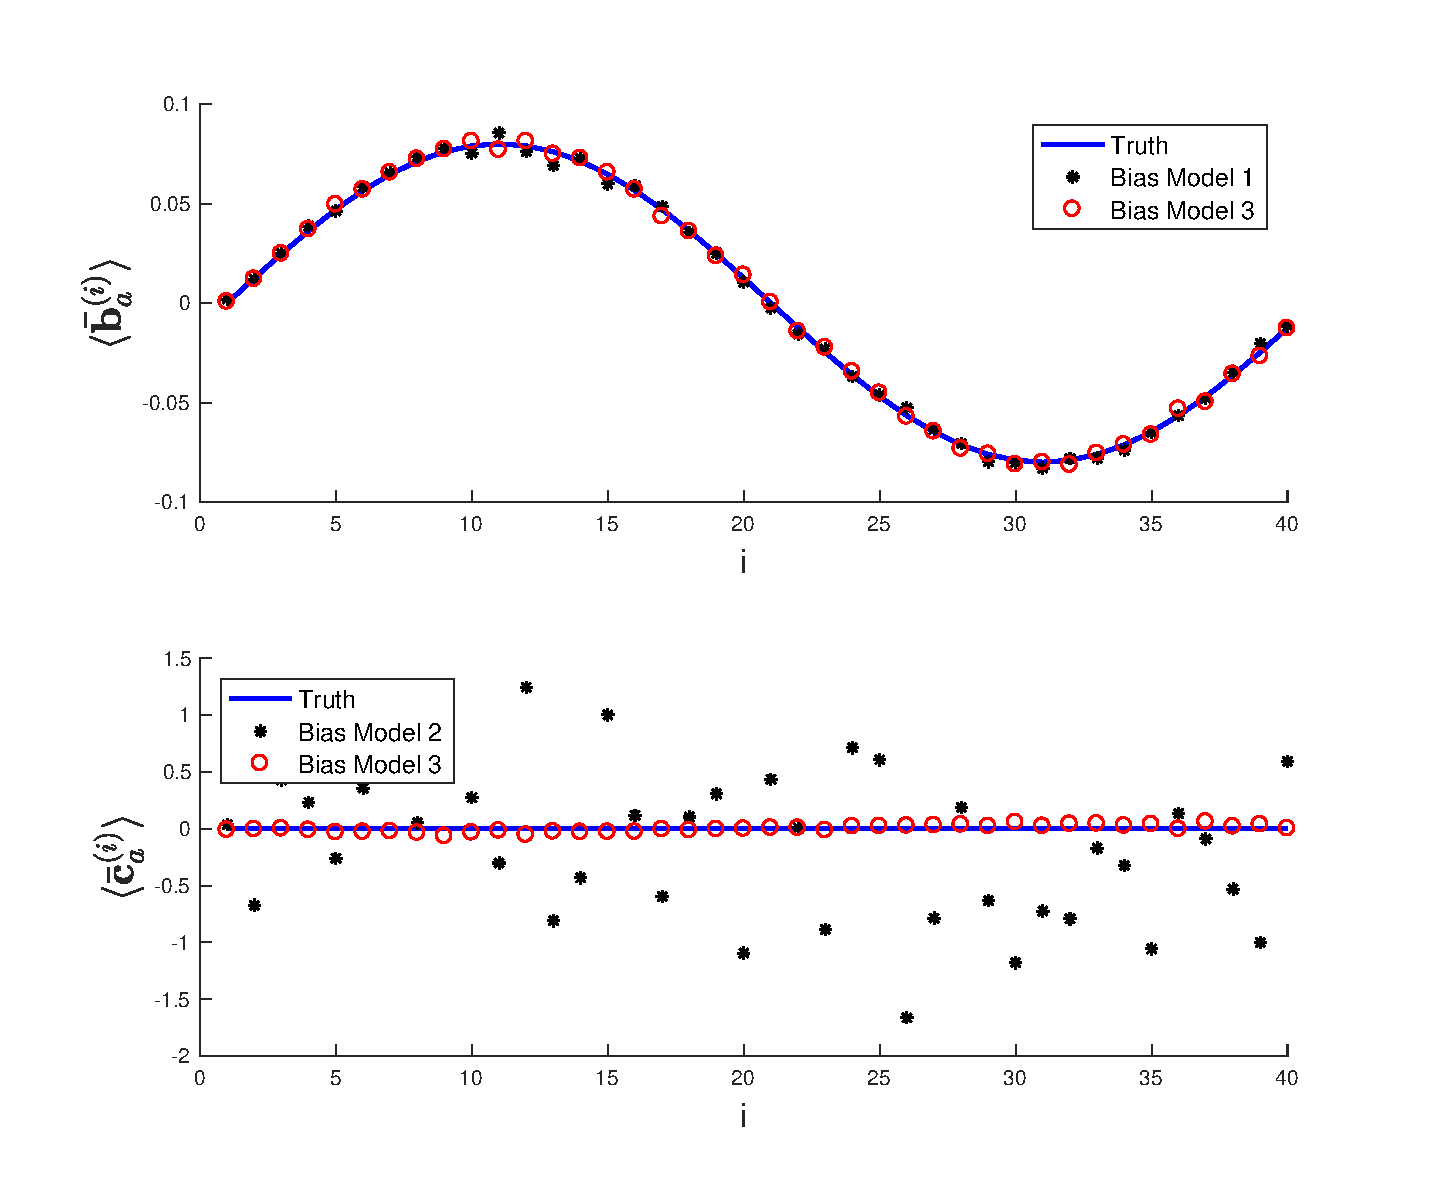
\includegraphics[scale=0.3]{Figures/BiasEstM1}
\caption{Time-averaged bias estimate at each location for the case with Type I model error. The truth $\zeta_i\Delta t$ and $-\xi_i$ are shown as the solid curve.}
\label{BiasEstM1}
\end{figure}
\subsubsection{Type II Model Bias}
In this experiment, we perform data assimilation using the model without bias estimation with unaugmented states i.e. eq.(\ref{lorenz}), and the three models with augmented space defined in subsection \ref{models}, when the true state is evolved with Type II model error, defined in eq.(\ref{error2}), with $B=0.2F=1.6$ in eq.(\ref{Bdef}).
\paragraph{Settling time of error}
The behavior of error with respect to time in this case is similar but still different from that of Type I model bias. Fig.(\ref{ErrVsTimeM2.1}) shows that the error for model 3 converges rather rapidly. However, the error for model 2, which best captures the dynamics, stabilizes after a rather long time. Some has suggested using a larger initial spread will reduce the settling time, but the improvement is small. We will accordingly use 400 as number of time steps in the experiment below, and time step 200 to 400 as the period for time averaging.
\begin{figure} 
\centering
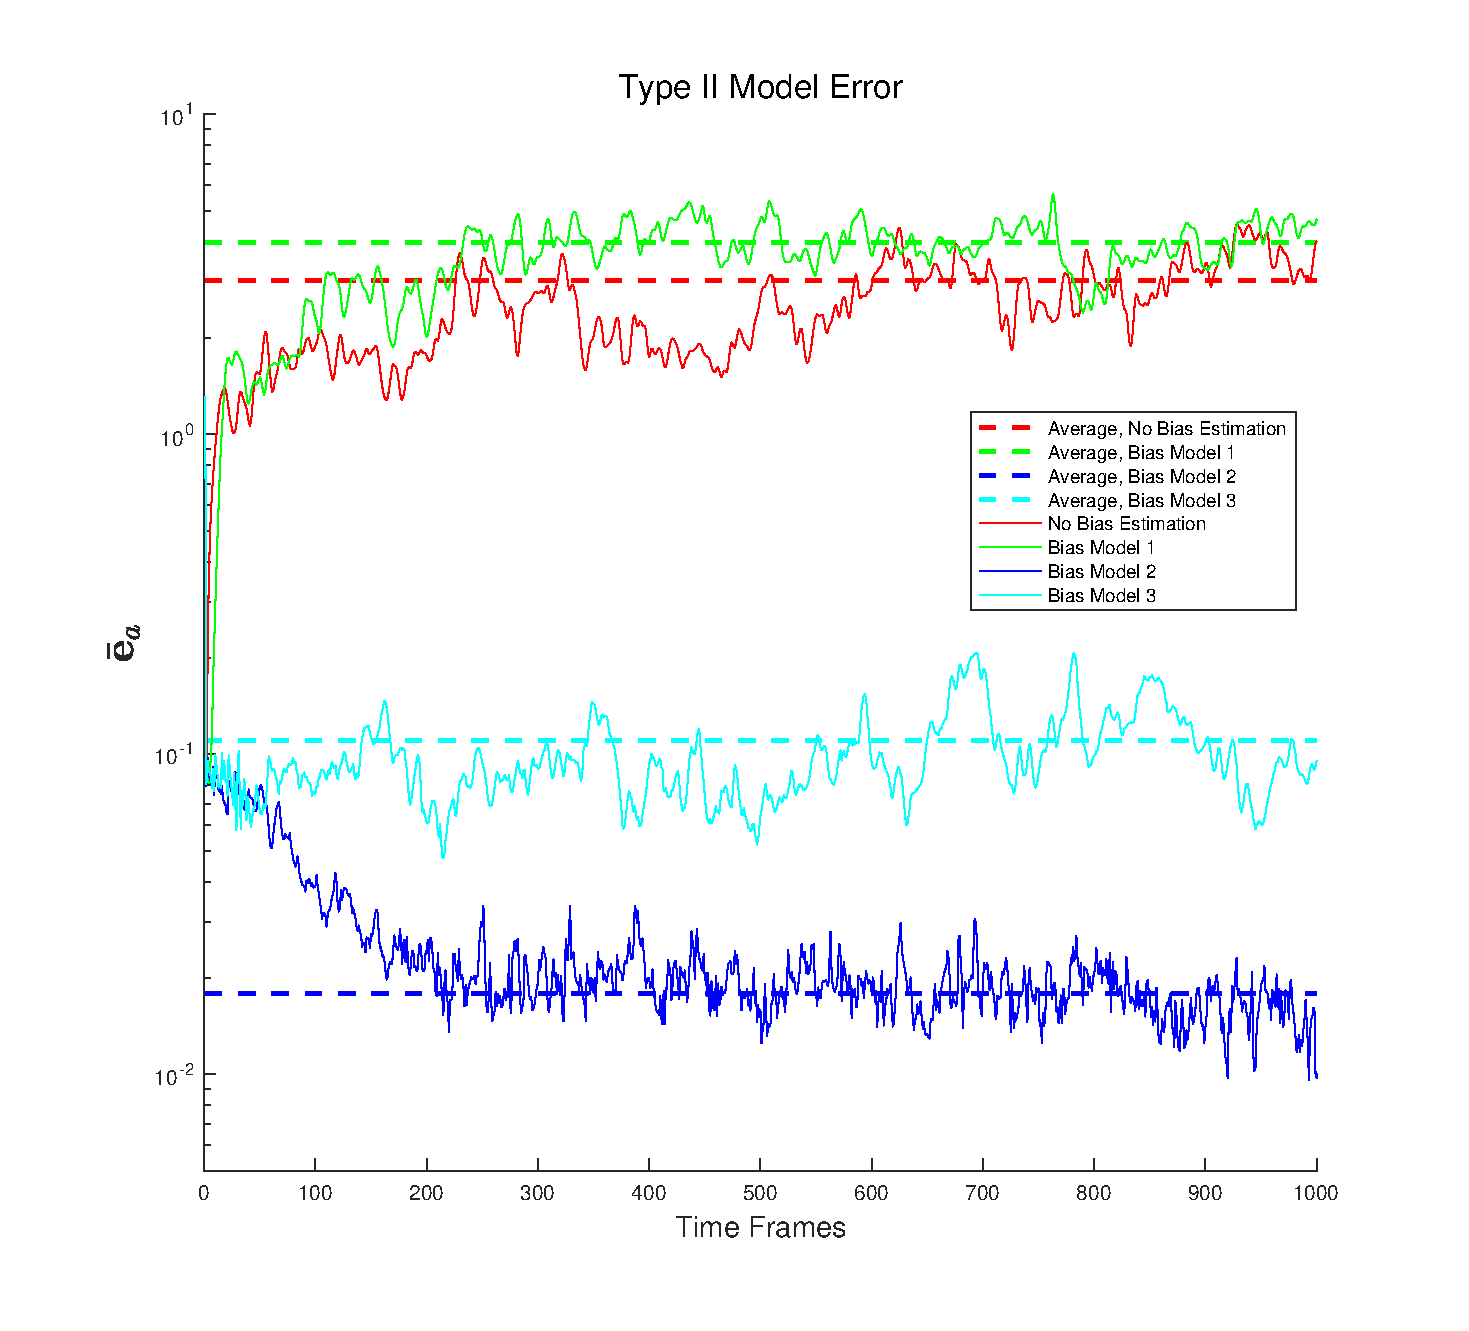
\includegraphics[scale=0.3]{Figures/ErrVsTimeM2_1}
\caption{Time-averaged rms analysis error, $\langle\langle\bar{\pmb{e}}_a\rangle\rangle$, and rms analysis error at each time step $\bar{\pmb{e}}_a^{(n)}$, for the Type II model error, with all 4 models.}
\label{ErrVsTimeM2.1}
\end{figure}
\paragraph{Performance with $\mu$}
Fig.(\ref{AErrVsMuM2.1}) shows the relation between error and $\mu$. Similar to the case of Type I model bias, the models that are formulated to account for the Type II model bias perform better than those that do not account for this type of model bias. Model 2 performs the best. Model 3 performs worse than model 2, but still significantly better than the others, probably since model 3 introduces unnecessary parameters $\pmb{c}$ in this case. We can see that for model 2, we can safely say there exist an optimal value for $\mu$ around $0.4$, which is very similar to the case in the perfect model. For the other models, larger value of $\mu$ seems to improve the performance, especially for the perfect model and bias model 1.
\begin{figure} 
\centering
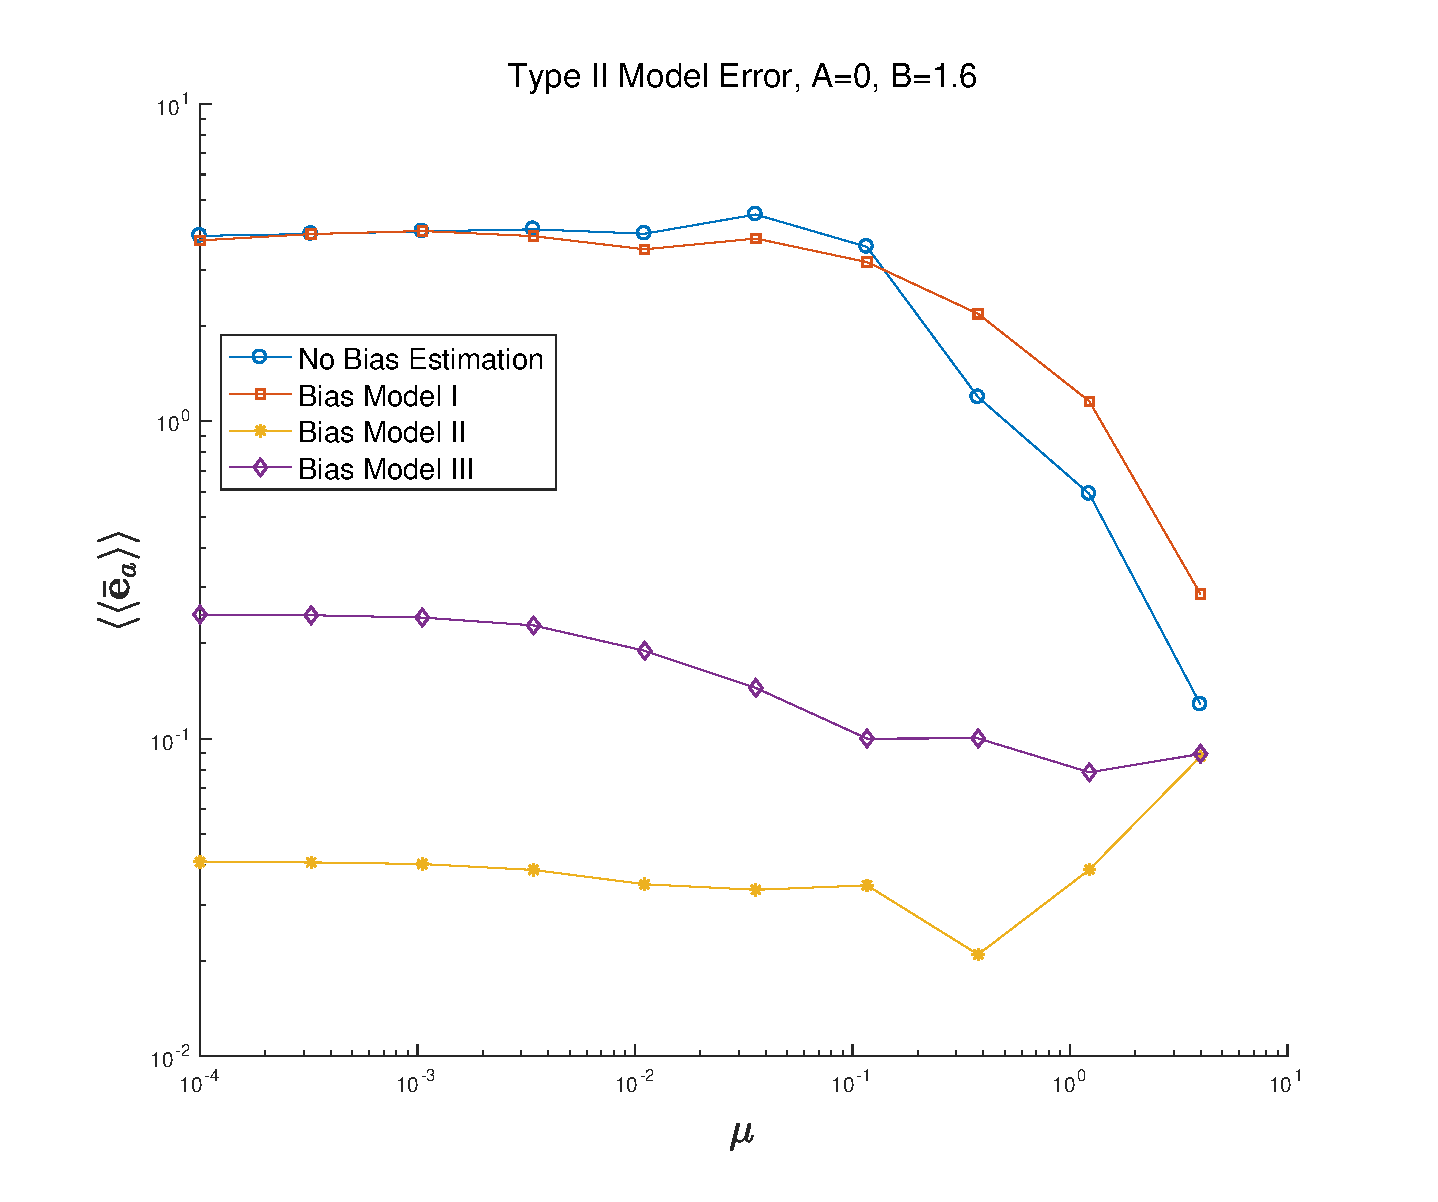
\includegraphics[scale=0.3]{Figures/AErrVsMuM2_1}
\caption{Time-averaged rms analysis error, $\langle\langle\bar{\pmb{e}}_a\rangle\rangle$, versus the variance inflation parameter $\mu$, for the Type II model error, with all 4 models.}
\label{AErrVsMuM2.1}
\end{figure}
\paragraph{Bias estimation}
Fig.(\ref{BiasEstM2}) shows the results for bias estimation. The analysis of the results is basically the same as that of Type I model bias. Both model 2 and 3 capture the bias very well, with very few noticeable deviance from the truth. And model 3 also provides good estimation for the zero "bias", whereas model 1 fails to do so.
\begin{figure} 
\centering
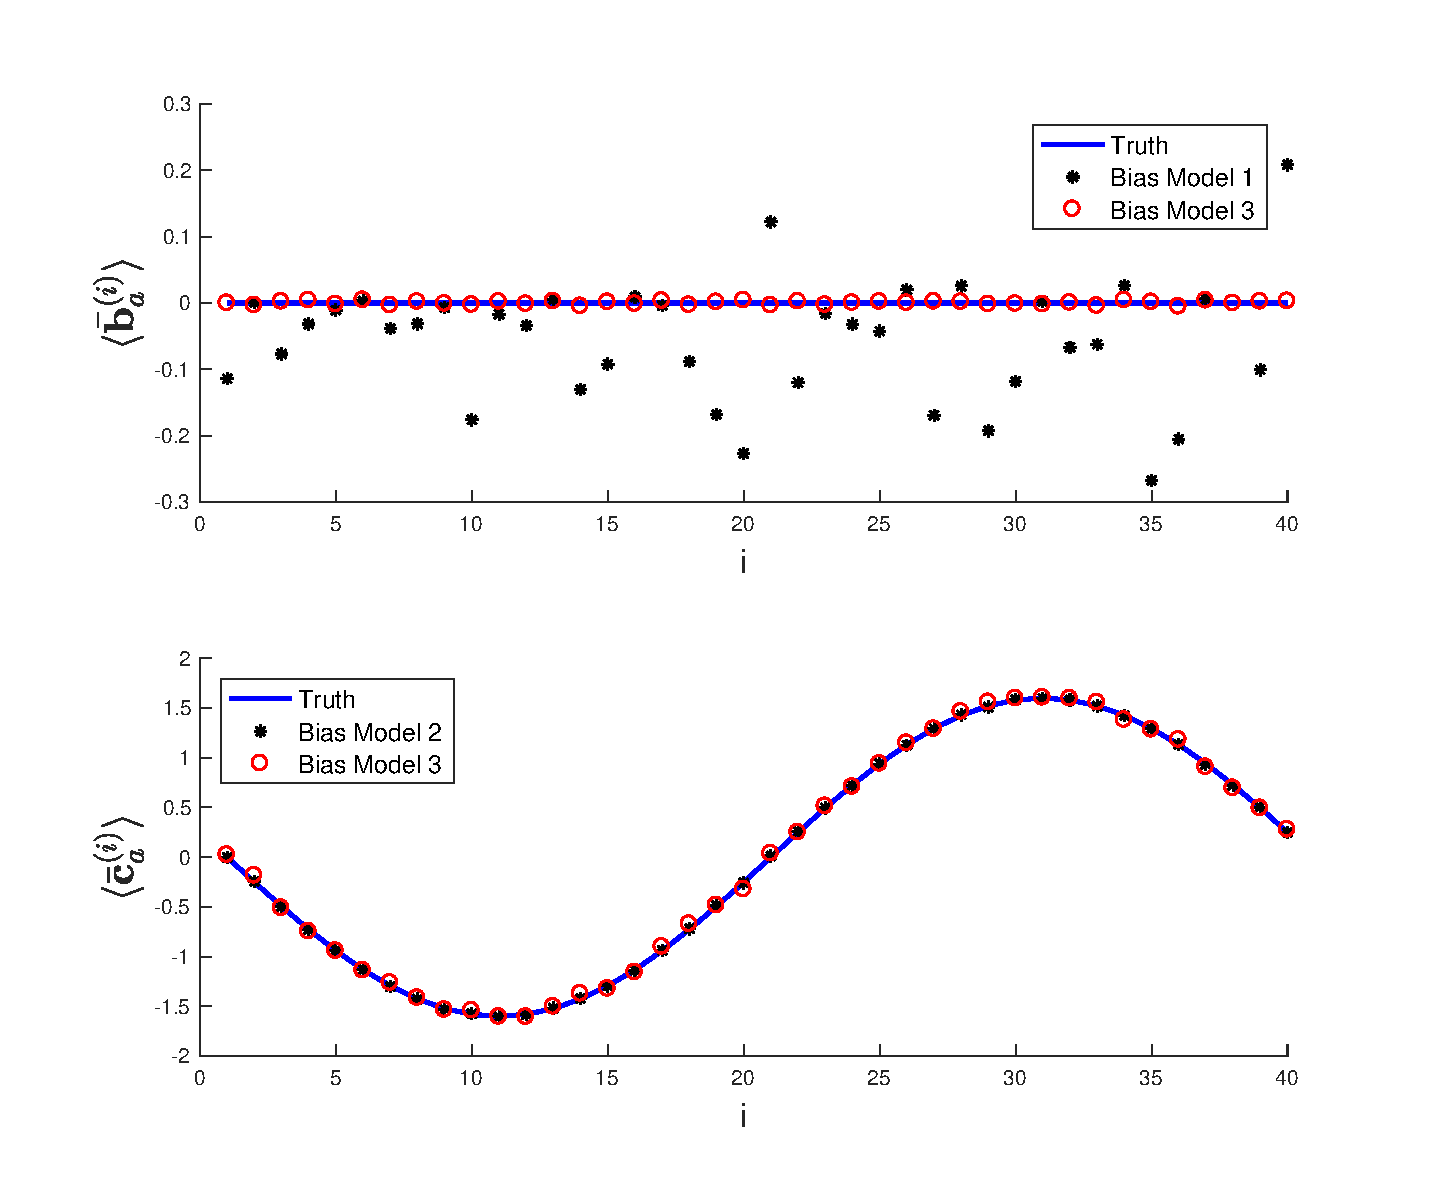
\includegraphics[scale=0.3]{Figures/BiasEstM2}
\caption{Time-averaged bias estimate at each location for the case with Type II model error. The truth $\zeta_i\Delta t$ and $-\xi_i$ are shown as the solid curve.}
\label{BiasEstM2}
\end{figure}
\subsubsection{Type III Model Bias}
In this experiment, we perform data assimilation using the model without bias estimation with unaugmented states i.e. eq.(\ref{lorenz}), and the three models with augmented space defined in subsection \ref{models}, when the true state is evolved with Type I model error, defined in eq.(\ref{error3}), with $A=0.2F=1.6$ in eq.(\ref{Adef}) and $B=0.2F=1.6$ in eq.(\ref{Bdef}).
\paragraph{Settling time of error}
The behavior of error with respect to time in this case is really similar as the case of Type I model bias. Fig.(\ref{ErrVsTimeM3.1}) shows that the error for model 3 converges rather rapidly, and for other models, which do not capture some aspect of the model error, the error is initially small, takes a long time to increase and finally stay stable around a large value. We will use 200 as number of time steps in the experiment below, and time step 100 to 200 as the period for time averaging.
\begin{figure} 
\centering
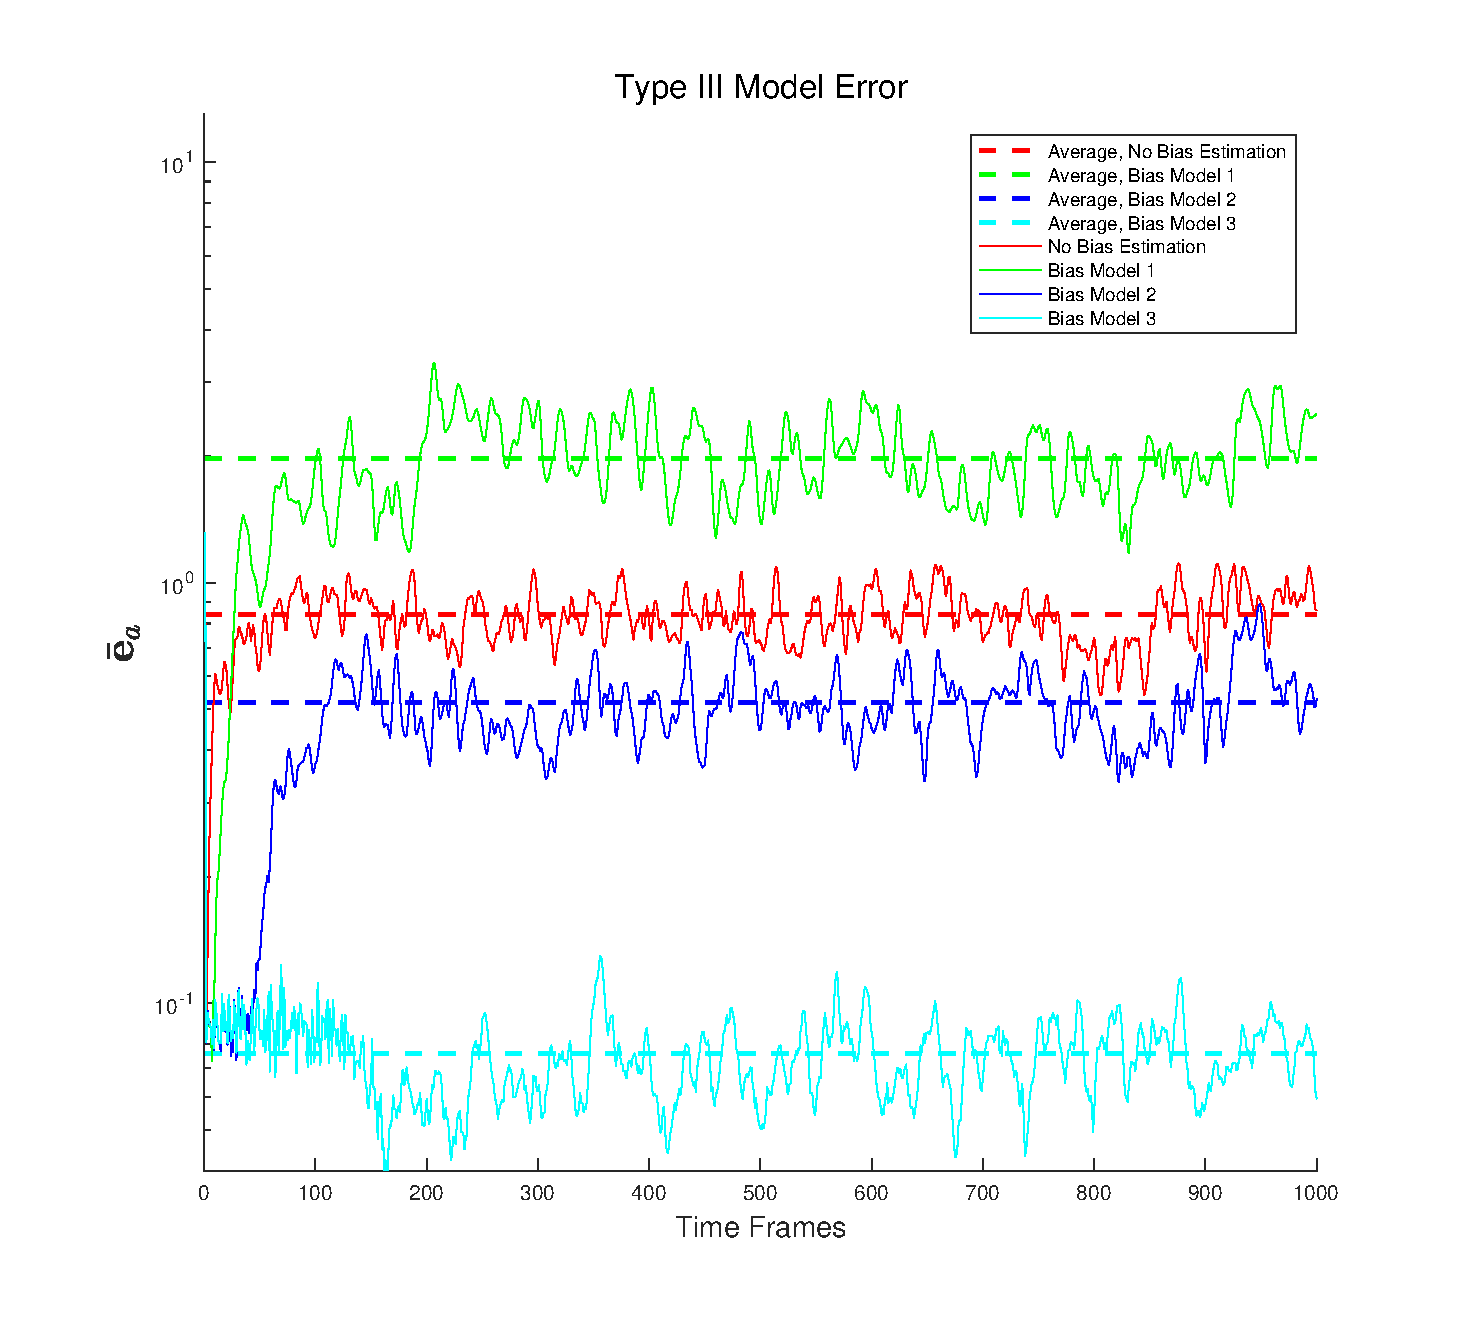
\includegraphics[scale=0.3]{Figures/ErrVsTimeM3_1}
\caption{Time-averaged rms analysis error, $\langle\langle\bar{\pmb{e}}_a\rangle\rangle$, and rms analysis error at each time step $\bar{\pmb{e}}_a^{(n)}$, for the Type III model error, with all 4 models.}
\label{ErrVsTimeM3.1}
\end{figure}
\paragraph{Performance with $\mu$}
Fig.(\ref{AErrVsMuM3.1}) shows the relation between error and $\mu$ in this case. We notice that the plot is quite different from those of Type I and II model bias. For a range of values for $\mu$, model 3, which is supposed to capture the dynamics the best, performs significantly better than other models. However, as we increase $\mu$, the performance of all models is improved, and eventually, at $\mu=4$, the advantage for model 3 is not as apparent, though still a little bit better than the model without bias estimation. Also, the minimum error achieved is considerably larger than those of the previous cases. One way to explain this is: although model 3 is formulated such that it includes all the bias parameters, the actual effect of mixture of the two types of model error is complicated than we initially think.
\begin{figure} 
\centering
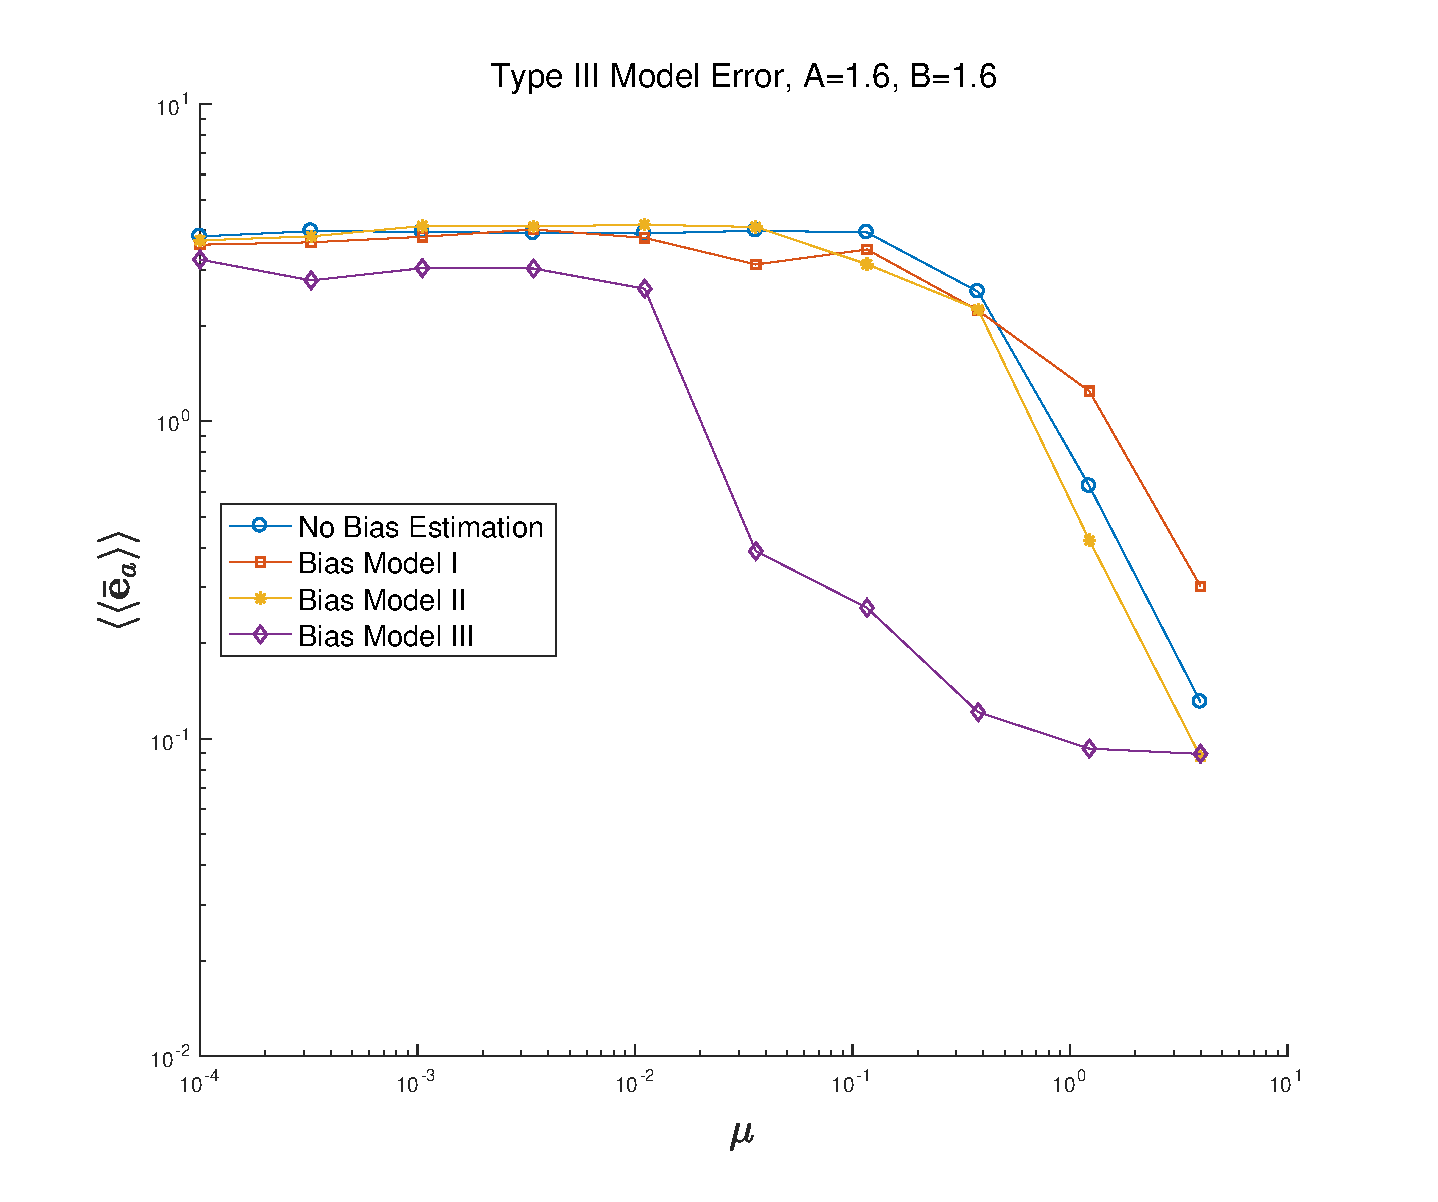
\includegraphics[scale=0.3]{Figures/AErrVsMuM3_1}
\caption{Time-averaged rms analysis error, $\langle\langle\bar{\pmb{e}}_a\rangle\rangle$, versus the variance inflation parameter $\mu$, for the Type III model error, with all 4 models.}
\label{AErrVsMuM3.1}
\end{figure}
\paragraph{Bias estimation}
Fig.(\ref{BiasEstM3}) shows the results for bias estimation. Although model 3 does not significantly outperform the other models in terms of time-averaged rms error, it does capture the bias remarkably well. The estimation essentially overlaps the truth. Meanwhile, model 1 completely fails to estimate $\pmb{\zeta}$, and the estimation of $\pmb{\xi}$ by model 2 is also much worse than that by model 3. This might suggest that model 3 is still potentially the best model for Type III model error, and we need to devise a better algorithm, or a different form of bias model, based on model 3, to improve the performance.
\begin{figure} 
\centering
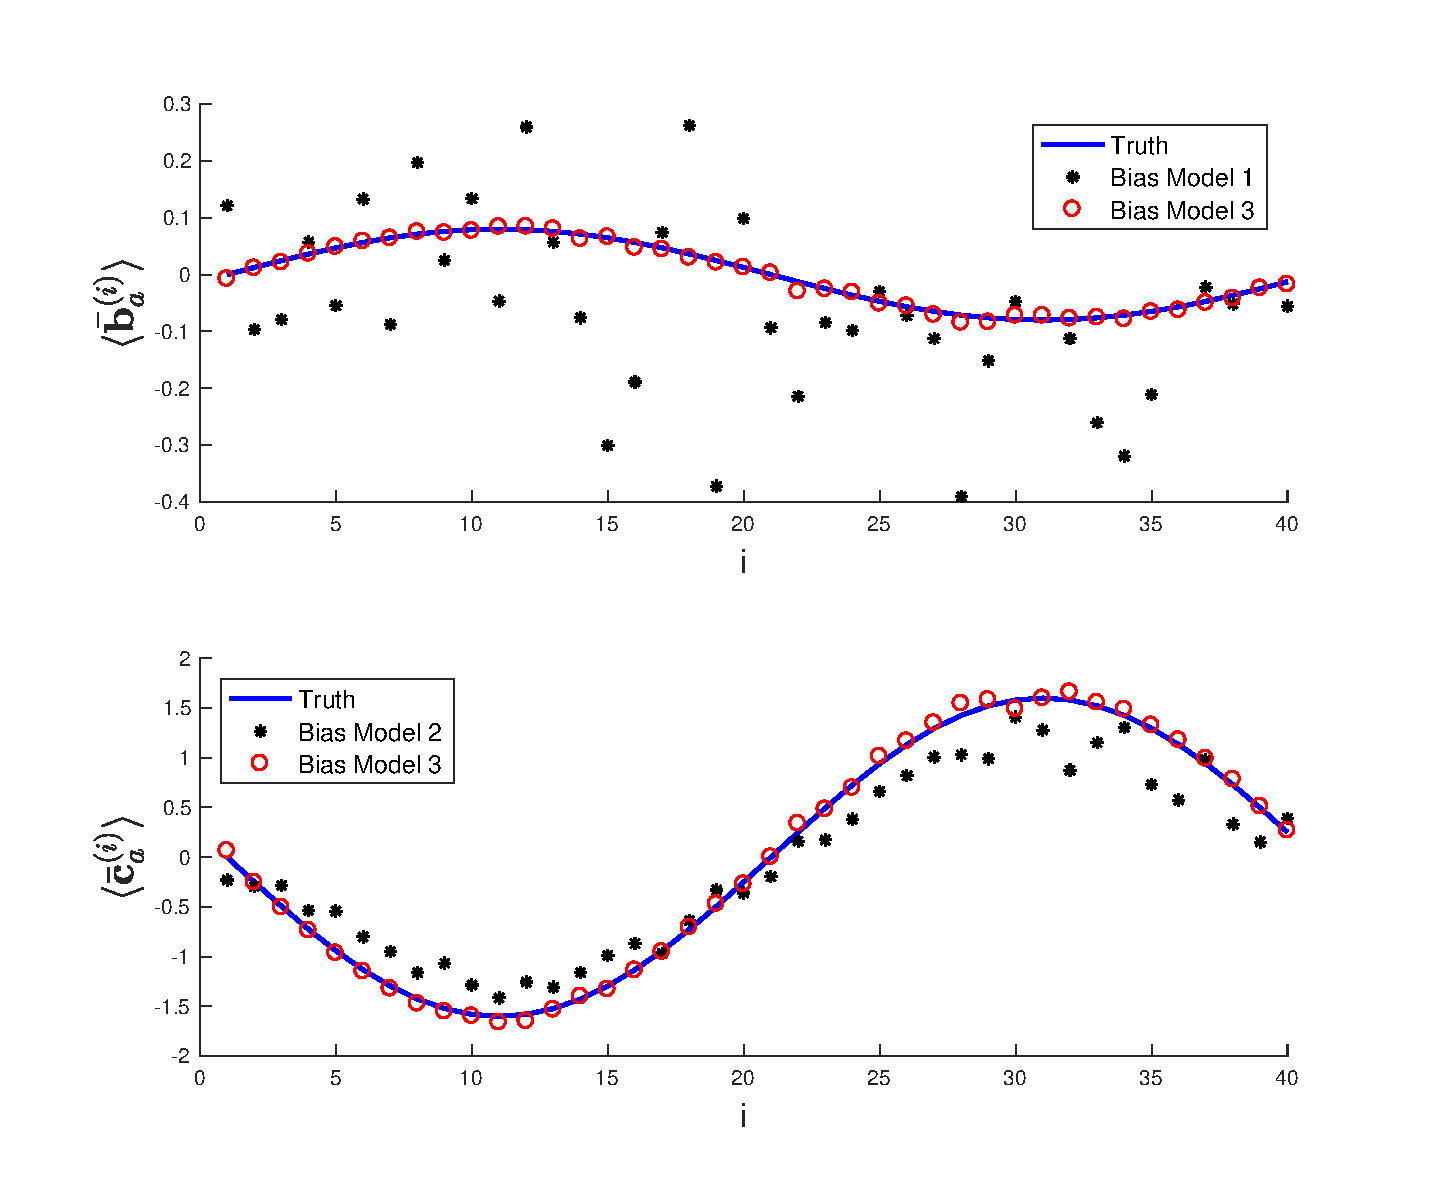
\includegraphics[scale=0.3]{Figures/BiasEstM3}
\caption{Time-averaged bias estimate at each location for the case with Type III model error. The truth $\zeta_i\Delta t$ and $-\xi_i$ are shown as the solid curve.}
\label{BiasEstM3}
\end{figure}
\subsection{Conclusions}
We considered three bias models for use in state space augmentation strategies to account for the three types of model error.\\
We find out the performance of data assimilation strongly depends on the specific type of model error and the specific model used for state augmentation. Generally speaking, if a model is formulated to account for certain type of error, than in the case with that type of error, the model will outperform other models. However, if the model error is complicated, then the advantage is not as apparent.\\
Moreover, we find out that the inflation coefficient $\mu$ plays an important role in determining the performance. Generally speaking, the less confidence we have for the model, or the farther from the truth the model is, or the larger the model error is, the larger $\mu$ we should use. Nevertheless, if the model is really close to the truth, or if the model captures the dynamics really well, then we should choose $\mu$ carefully; in many cases, the optimal $\mu$ exists in a relatively small range.
\end{document}
